\subsection{The Windows API}\label{section:background windows api}
To interact with the Windows operating system (e.g. write to a file), applications need to call functions provided by Windows. These functions (and related data structures) are collectively called the Windows API. The API is documented online\footnote{\tiny \url{https://docs.microsoft.com/en-us/windows/win32/api/_winprog/}}.

In \autoref{chapter:persistence techniques} and \autoref{chapter:call signatures}, we will see that malware calls specific API functions to achieve persistence.

\autoref{listing:windows API example} shows a simple example program that writes text to a file\footnote{The Windows API uses its own types to represent C types. For example, \texttt{DWORD} is the API type for a 32-bit unsigned integer.}. It calls three functions to interact with Windows: \texttt{CreateFile}\footnote{\tiny \url{https://docs.microsoft.com/en-us/windows/win32/api/fileapi/nf-fileapi-createfilew}}, \texttt{WriteFile}\footnote{\tiny \url{https://docs.microsoft.com/en-us/windows/win32/api/fileapi/nf-fileapi-writefile}} and \texttt{CloseHandle}\footnote{\tiny \url{https://docs.microsoft.com/en-us/windows/win32/api/handleapi/nf-handleapi-closehandle}}.

\begin{minipage}{0.9\textwidth}
\begin{lstlisting}[caption={An example of creating and writing to a file using the Windows API.}, captionpos=b, label={listing:windows API example}]
#include <iostream>
#include <windows.h>

int main() {
	HANDLE hFile;

	LPCWSTR filename = L"test.txt";
	LPCWSTR buffer = L"Hello World";
	DWORD szBuffer = wcslen(buffer) * sizeof(WCHAR);

	hFile = CreateFile(
		filename,
		GENERIC_WRITE,
		0,
		NULL,
		CREATE_ALWAYS,
		FILE_ATTRIBUTE_NORMAL,
		0);
	WriteFile(
		hFile,
		(LPVOID) buffer,
		szBuffer,
		0,
		NULL);
	CloseHandle(hFile);

	return 0;
}
\end{lstlisting}
\end{minipage}

\subsubsection{Dynamic-link Libraries}\label{section:dlls}
The functions in the Windows API are provided in dynamic-link libraries (DLLs), executables that do not run by themselves. They export functions that can be used by other applications. Dynamic-link libraries offer multiple advantages over statically linked libraries. Most notably, functions do not have to be compiled into every executable that uses them and need to be loaded into memory only once.

\subsubsection{Calling API Functions}\label{section:background calling api functions}
As we can see in \autoref{listing:windows API example}, Windows API functions are called like any other function. The process of matching a function call to the correct address is handled by Windows and transparent to developers.

Executables have an \emph{Import Address Table} (IAT), which is used to translate external function calls in the executable to the actual addresses of the functions in memory. When a function in a DLL is called, the \texttt{call} instruction jumps to an address in the IAT, which in turn jumps to the actual address of the function. At load-time (i.e. when an executable is loaded into memory before executing it), Windows adds the actual memory addresses of the functions to the IAT. This process is called \emph{load-time dynamic linking} \cite{load-time-dynamic-linking}.

It is also possible to load external functions at run-time (i.e. during the execution of an application), called \emph{run-time dynamic linking}. This requires developers to write their own code that finds the right address to a function at run-time. The Windows API provides two functions that help developers do this: \texttt{LoadLibrary} \footnote{\tiny \url{https://docs.microsoft.com/en-us/windows/win32/api/libloaderapi/nf-libloaderapi-loadlibrarya}} and \texttt{GetProcAddress}\footnote{\tiny \url{https://docs.microsoft.com/en-us/windows/win32/api/libloaderapi/nf-libloaderapi-getprocaddress}}. They work like this:

\begin{enumerate}
    \item \texttt{LoadLibrary} is called to get a handle on the DLL that contains the required function.
    \item \texttt{GetProcAddress} is called to search for the required function using the handle to the DLL.
\end{enumerate}

Malware authors prefer to load functions at run-time because the functions are not added to the IAT, which hides the external functions they make use of.

\subsubsection{A Comparison of Load-Time Dynamic Linking \& Run-time Dynamic Linking}\label{section:comparison load time run time dynamic linking}
\autoref{appendix:source code run time linking} contains the source code of two executables. The executables are semantically equivalent, but \autoref{listing:load-time dynamic linking code} uses direct function calls to Windows API and \autoref{listing:run-time dynamic linking code} uses run-time dynamic linking. Both executables perform the following steps:

\begin{enumerate}
    \item Open the Windows Registry key \path{HKLM\SOFTWARE\Microsoft\Windows NT\CurrentVersion}, by calling \texttt{RegOpenKeyEx}\footnote{\tiny \url{https://docs.microsoft.com/en-us/windows/win32/api/winreg/nf-winreg-regopenkeyexw}}.

    \item Get the data of the value \texttt{ProductName} in the Registry key, by calling \texttt{RegQueryValueEx}\footnote{\tiny \url{https://docs.microsoft.com/en-us/windows/win32/api/winreg/nf-winreg-regqueryvalueexw}}.

    \item Close the Registry key, by calling \texttt{RegCloseKey}\footnote{\tiny \url{https://docs.microsoft.com/en-us/windows/win32/api/winreg/nf-winreg-regclosekey}}.
\end{enumerate}

In \autoref{fig:call comparison}, we see the Assembly that is used to call \texttt{RegQueryValueEx} in both executables. We can see that the disassembler detected which function is being called in \autoref{fig:load-time linked API call}, but not in \autoref{fig:run-time linked API call}. The \texttt{call} instruction in \autoref{fig:run-time linked API call} does not jump to a static address, but to an address that is loaded into the \texttt{eax} register.

\begin{figure}[ht]
    \centering
    \begin{subfigure}[ht]{\textwidth}
        \centering
        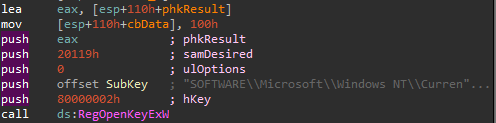
\includegraphics[width=0.7\textwidth]{resources/images/load_time_api_call_disassembler.png}
        \caption{A (load-time dynamically linked) call to \texttt{RegOpenKeyExW} (disassembled by IDA Pro).}
        \label{fig:load-time linked API call}
    \end{subfigure}
    \hfill
    \begin{subfigure}[ht]{\textwidth}
        \centering
        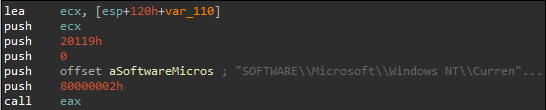
\includegraphics[width=0.7\textwidth]{resources/images/run_time_api_call_disassembler.png}
        \caption{A run-time dynamically linked call to \texttt{RegOpenKeyExW} (disassembled by IDA Pro).}
        \label{fig:run-time linked API call}
    \end{subfigure}
    \caption{A comparison of a load-time dynamically linked call and a run-time dynamically linked call to \texttt{RegOpenKeyExW}.}
    \label{fig:call comparison}
\end{figure}

In \autoref{fig:imports comparison}, we see part of the import table (decoded by IDA Pro) of the two executables. In \autoref{fig:load-time imports}, we see the three API functions, as expected. However, in \autoref{fig:run-time imports} we do not see the API functions, because the executable loads the functions itself.

\begin{figure}[ht]
    \centering
    \begin{subfigure}[ht]{\textwidth}
        \centering
        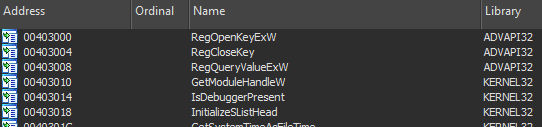
\includegraphics[width=0.7\textwidth]{resources/images/load_time_api_call_imports.png}
        \caption{The imports of \autoref{listing:load-time dynamic linking code} using load-time dynamically linked calls.}
        \label{fig:load-time imports}
    \end{subfigure}
    \hfill
    \begin{subfigure}[ht]{\textwidth}
        \centering
        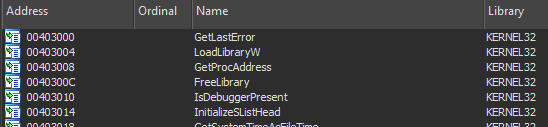
\includegraphics[width=0.7\textwidth]{resources/images/run_time_api_call_imports.png}
        \caption{The imports of \autoref{listing:run-time dynamic linking code} using run-time dynamically linked calls.}
        \label{fig:run-time imports}
    \end{subfigure}
    \caption{A comparison of the import address table of two executables.}
    \label{fig:imports comparison}
\end{figure}
